% Created 2022-04-19 mar 19:08
% Intended LaTeX compiler: pdflatex
\documentclass[11pt]{article}
\usepackage[utf8]{inputenc}
\usepackage[T1]{fontenc}
\usepackage{graphicx}
\usepackage{grffile}
\usepackage{longtable}
\usepackage{wrapfig}
\usepackage{rotating}
\usepackage[normalem]{ulem}
\usepackage{amsmath}
\usepackage{textcomp}
\usepackage{amssymb}
\usepackage{capt-of}
\usepackage{hyperref}
\usepackage[spanish]{babel}
\usepackage{svg}
\makeatletter
\usepackage{fancyhdr}
\usepackage{fancyvrb}
\usepackage{tcolorbox}
\usepackage{listings, caption, xcolor}
\author{Luis Eduardo Galindo Amaya}
\date{\textit{[2022-04-19 mar]}}
\title{Práctica 8\\\medskip
\large Relaciones Entre Clases}
\hypersetup{
 pdfauthor={Luis Eduardo Galindo Amaya},
 pdftitle={Práctica 8},
 pdfkeywords={},
 pdfsubject={},
 pdfcreator={Emacs 26.3 (Org mode 9.1.9)}, 
 pdflang={Spanish}}
\begin{document}

\pagestyle{fancy}
\fancyhf{}
\lhead{Luis Eduardo Galindo Amaya}
\rhead{Programación orientada a Objetos}
\cfoot{\thepage}


\begin{titlepage}
\centering
{\bfseries\LARGE Universidad Autonoma \par de Baja California \par}
\vfill
{\scshape\Huge \@title \par}
\vfill
\begin{center}

\includegraphics[width=4cm]{../0imports/img/logo}
\end{center}
\vfill
{\Large Autor: \par}
{\Large \@author \par}
1274895
\vfill
{\Large \today \par}
\end{titlepage}


\definecolor{backcolour}{rgb}{0.95,0.95,0.92}

\lstset{    
  backgroundcolor=\color{backcolour},   
%  frame=top,
%  frame=bottom,
  numbers=left,
  basicstyle=\ttfamily,
  stepnumber=1,                           
  numbersep=10pt,                         
  tabsize=2,                              
  extendedchars=true,                     
  breaklines=true,
  captionpos=t,   
  mathescape=true,
  stringstyle=\color{white}\ttfamily, 
  showspaces=false,     
  showtabs=false,       
  xleftmargin=17pt,
  framexleftmargin=17pt,
%  framexrightmargin=17pt,
  framexbottommargin=5pt,
  framextopmargin=5pt,
  showstringspaces=false,
  numberstyle=\tiny\ttfamily
 }

\captionsetup[lstlisting]{
format=listing,
singlelinecheck=false, 
margin=0pt,
labelfont=bf
}

\renewcommand{\lstlistingname}{Programa}% Listing -> Algorithm

\section*{Fotos}
\label{sec:org8df62d9}
\begin{center}
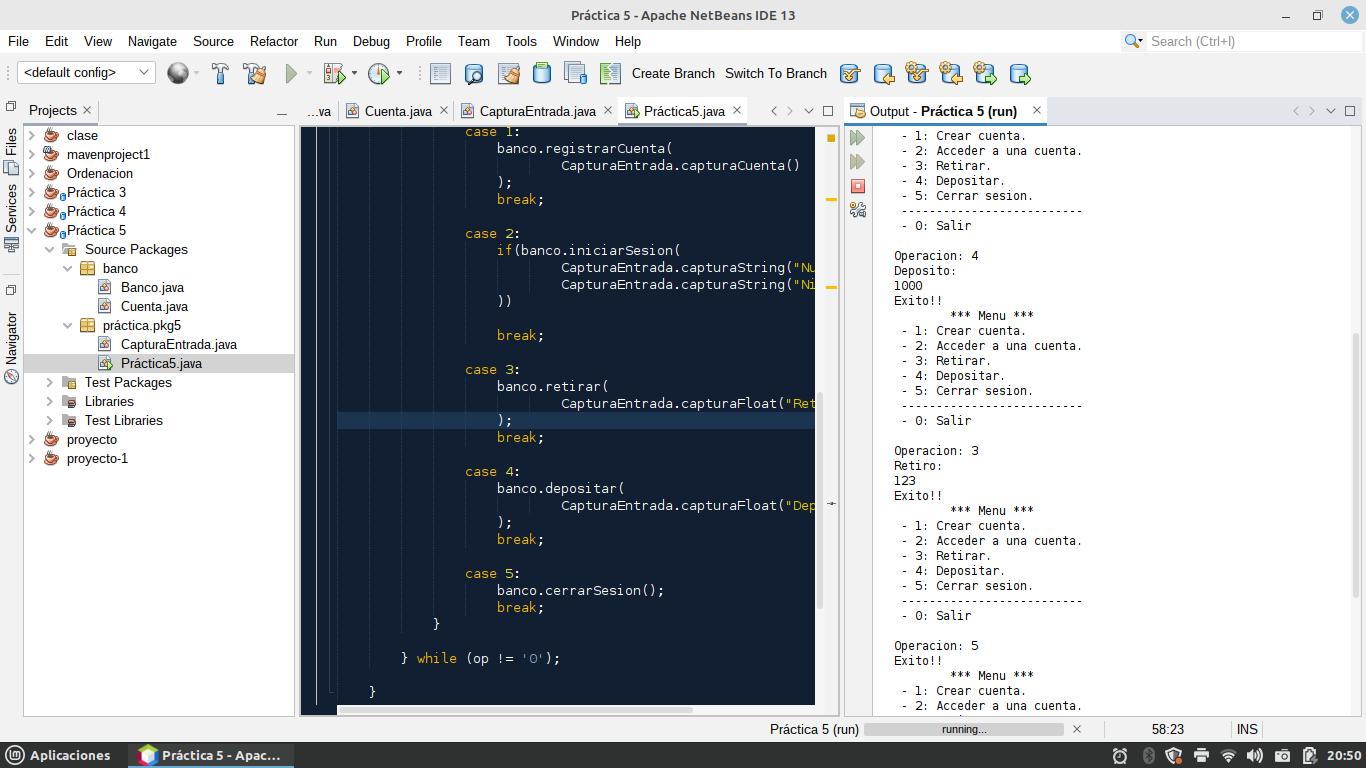
\includegraphics[width=.9\linewidth]{img/2.png}
\end{center}

\section*{Código}
\label{sec:orgf863f44}
\lstinputlisting[caption=main.py]{./src/Equipo.py}
\lstinputlisting[caption=Equipo.py]{./src/Equipo.py}
\lstinputlisting[caption=Jugador.py]{./src/Jugador.py}
\lstinputlisting[caption=Torneo.py]{./src/Torneo.py}

\section*{UML}
\label{sec:org49876a0}
\begin{center}
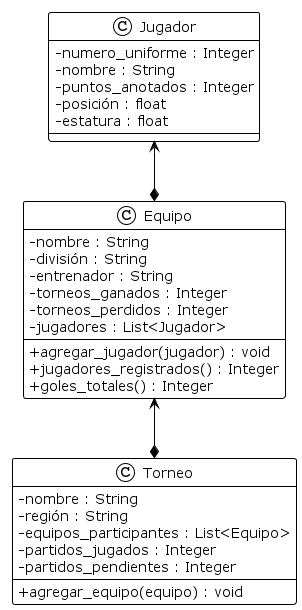
\includegraphics[width=150px]{img/uml.png}
\end{center}
\end{document}
